\chapter{Diseño e implementación}
\label{cap:disenoEImpl}
En este capítulo se explican todos los conceptos y decisiones que se han considerado relevantes para el diseño de la aplicación, así como el proceso de implementación diviendo la aplicación por bloques funcionales.

\section{Diseño}
El objetivo en lo relativo al diseño en Profinder era crear una aplicación escalable a distintos idiomas, con una experiencia de usuario agradable, bonita a la vista y que se ajustara a los principios \textit{open source}. A continuación se explica en detalle como se han intentado lograr estos objetivos.

\subsection{Experiencia de usuario}
Para conseguir una buena experiencia de usuario, se han intentado seguir una serie de principios de diseño para aplicaciones. También se ha intentado mantener una paleta de colores homogénea en la aplicación usando material design (véase el apartado \ref{subsec:material_design}) y  unas interfaces de usuario minimalistas, a la vez que autoexplicativas, a continuación se explican algunas de las medidas que se han tomado para lograr los objetivos anteriores.
\begin{itemize}
    \item Para la nevegación a través de la aplicación se ha utilizado una \textit{bottom bar} (como se ve en la figura \ref{fig:ejemplo_bottombar}), este es un elemento típico en aplicaciones, lo que implica que culaquier usuario, aunque no haya utilizado la aplicación nunca, sabrá navegar por ella.
    \begin{figure}[h]
        \centering
        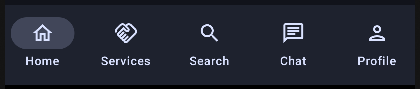
\includegraphics[width = 0.6\textwidth]{Imagenes/Fuentes/ejemplo_bottombar.png}
        \caption{Ejemplo de la bottom bar.}
        \label{fig:ejemplo_bottombar}
    \end{figure}
    \item La home es la pantalla principal de la aplicación, por lo que navegar a ella no puede implicar tener más de una pantalla entre medias, esto quiere decir que, desde cualquier pantalla de la aplicación debe ser posible ir a la home sin pulsar más de dos botones. 
    \item Las decisiones importantes a tomar en la aplicación deben ser ‘más dificiles’ en el sentido de que deben implicar más pasos para evitar que el usuario las tome por accidente. Un ejemplo de esto puede ser el cierre de sesiónya que el botón se encuentra en la esquina superior izquierda (más difícil de alcanzar con los pulgares) y al pulsarlo, se muestra un mensaje de confirmación. 
    \item Se ha trabajado en dar un buen feedback al usuario de las acciones realizadas en la aplicación, mostrando mensajes explicativos. También se ha intentado que el usuario sepa en todo momento lo que esta pasando, por ejemplo, mostrando pantallas de carga en los momentos de espera de datos. 
\end{itemize}

\subsection{Open source}
\label{subsec:openSource}
El código \textit{open source} (abierto, significando esto que el código desarrollado es público para cualquiera que lo quiera ver)
es un movimiento socio-tecnólogico que comenzó en la decada de 1980, cuando Richard Stallman (considerado por muchos el padre del movimiento de \textit{open source} o \textit{ free open source}, tomando la denotación de \textit{free} como libre no como gratuito) fundó la \textit{Free Software Foundation} (Fundación de código libre)\hyperlink{cap:biblio}{\endnote{\textbf{Free Software Foundation}: \url{https://www.fsf.org/}}}, así como el sitema operativo GNU\hyperlink{cap:biblio}{\endnote{\textbf{GNU}: \url{https://www.gnu.org/}}} (\textit{GNU's not Unix}). Richard creía que el software debía ser  creado de forma colaborativa y libremente compartido. Otro gran exponente de este movimiento (aunque con distintas motivaciones) fue el finlandés Linus Torwalds, creador del kernel Linux (GNU-Linux es el sistema operativo con el que se está escribiendo esta memoria y se ha realizado todo el proceso de desarrollo).

En este contexto, se ha intentado desarrollar Profinder siguiendo los principios \textit{open source} e intentando utilizar la mayor cantidad de herramientas de código abierto posible. Algunos ejemplos a parte de los que se han ido mencionando a lo largo de esta memoria pueden ser Firefox\hyperlink{cap:biblio}{\endnote{\textbf{Firefox}: \url{https://www.mozilla.org/es-ES/firefox/}}}, Neovim\hyperlink{cap:biblio}{\endnote{\textbf{Neovim}: \url{https://neovim.io/}}} y Linux\hyperlink{cap:biblio}{\endnote{\textbf{Linux}: \url{https://www.linux.org/pages/}}} entre otros. Asimismo se ha decidido que todo el código de este proyecto sea libre -siendo posible revisarlo, distribuirlo y modificarlo- así como el proceso seguido para hacerlo.

La mayoría del contenido en este apartado ha tomado las referencias del libro \textit{The Innovators} (Isaacson, 2015)\hyperlink{cap:biblio}{\endnote{\textit{The Innovators: How a Group of Hackers, Geniuses and Geeks Created the Digital Revolution}, Walter Isaacson, 2015}} 

\subsection{Idiomas}
Con el objetivo de hacer el proyecto lo mas ‘universal’ posible, el idioma principal utilizado para el desarrollo de Profinder (código, apuntes, \textit{commits}) ha sido el inglés. Sin embargo, todo los literales de texto que aparecen en la aplicación han sido incluidos en un archivo (\textit{strings.xml}) (en la figura \ref{fig:stringXml} se puede ver un ejemplo del mismo). El contenido de este fichero ha sido luego traducido al español, de tal forma que dependiendo del idioma del dispositivo del usuario, la aplicación estará en español o en inglés. Este mismo proceso podría ser llevado a cabo para añadir cualquier idioma.
\begin{figure}[h]
    \centering
    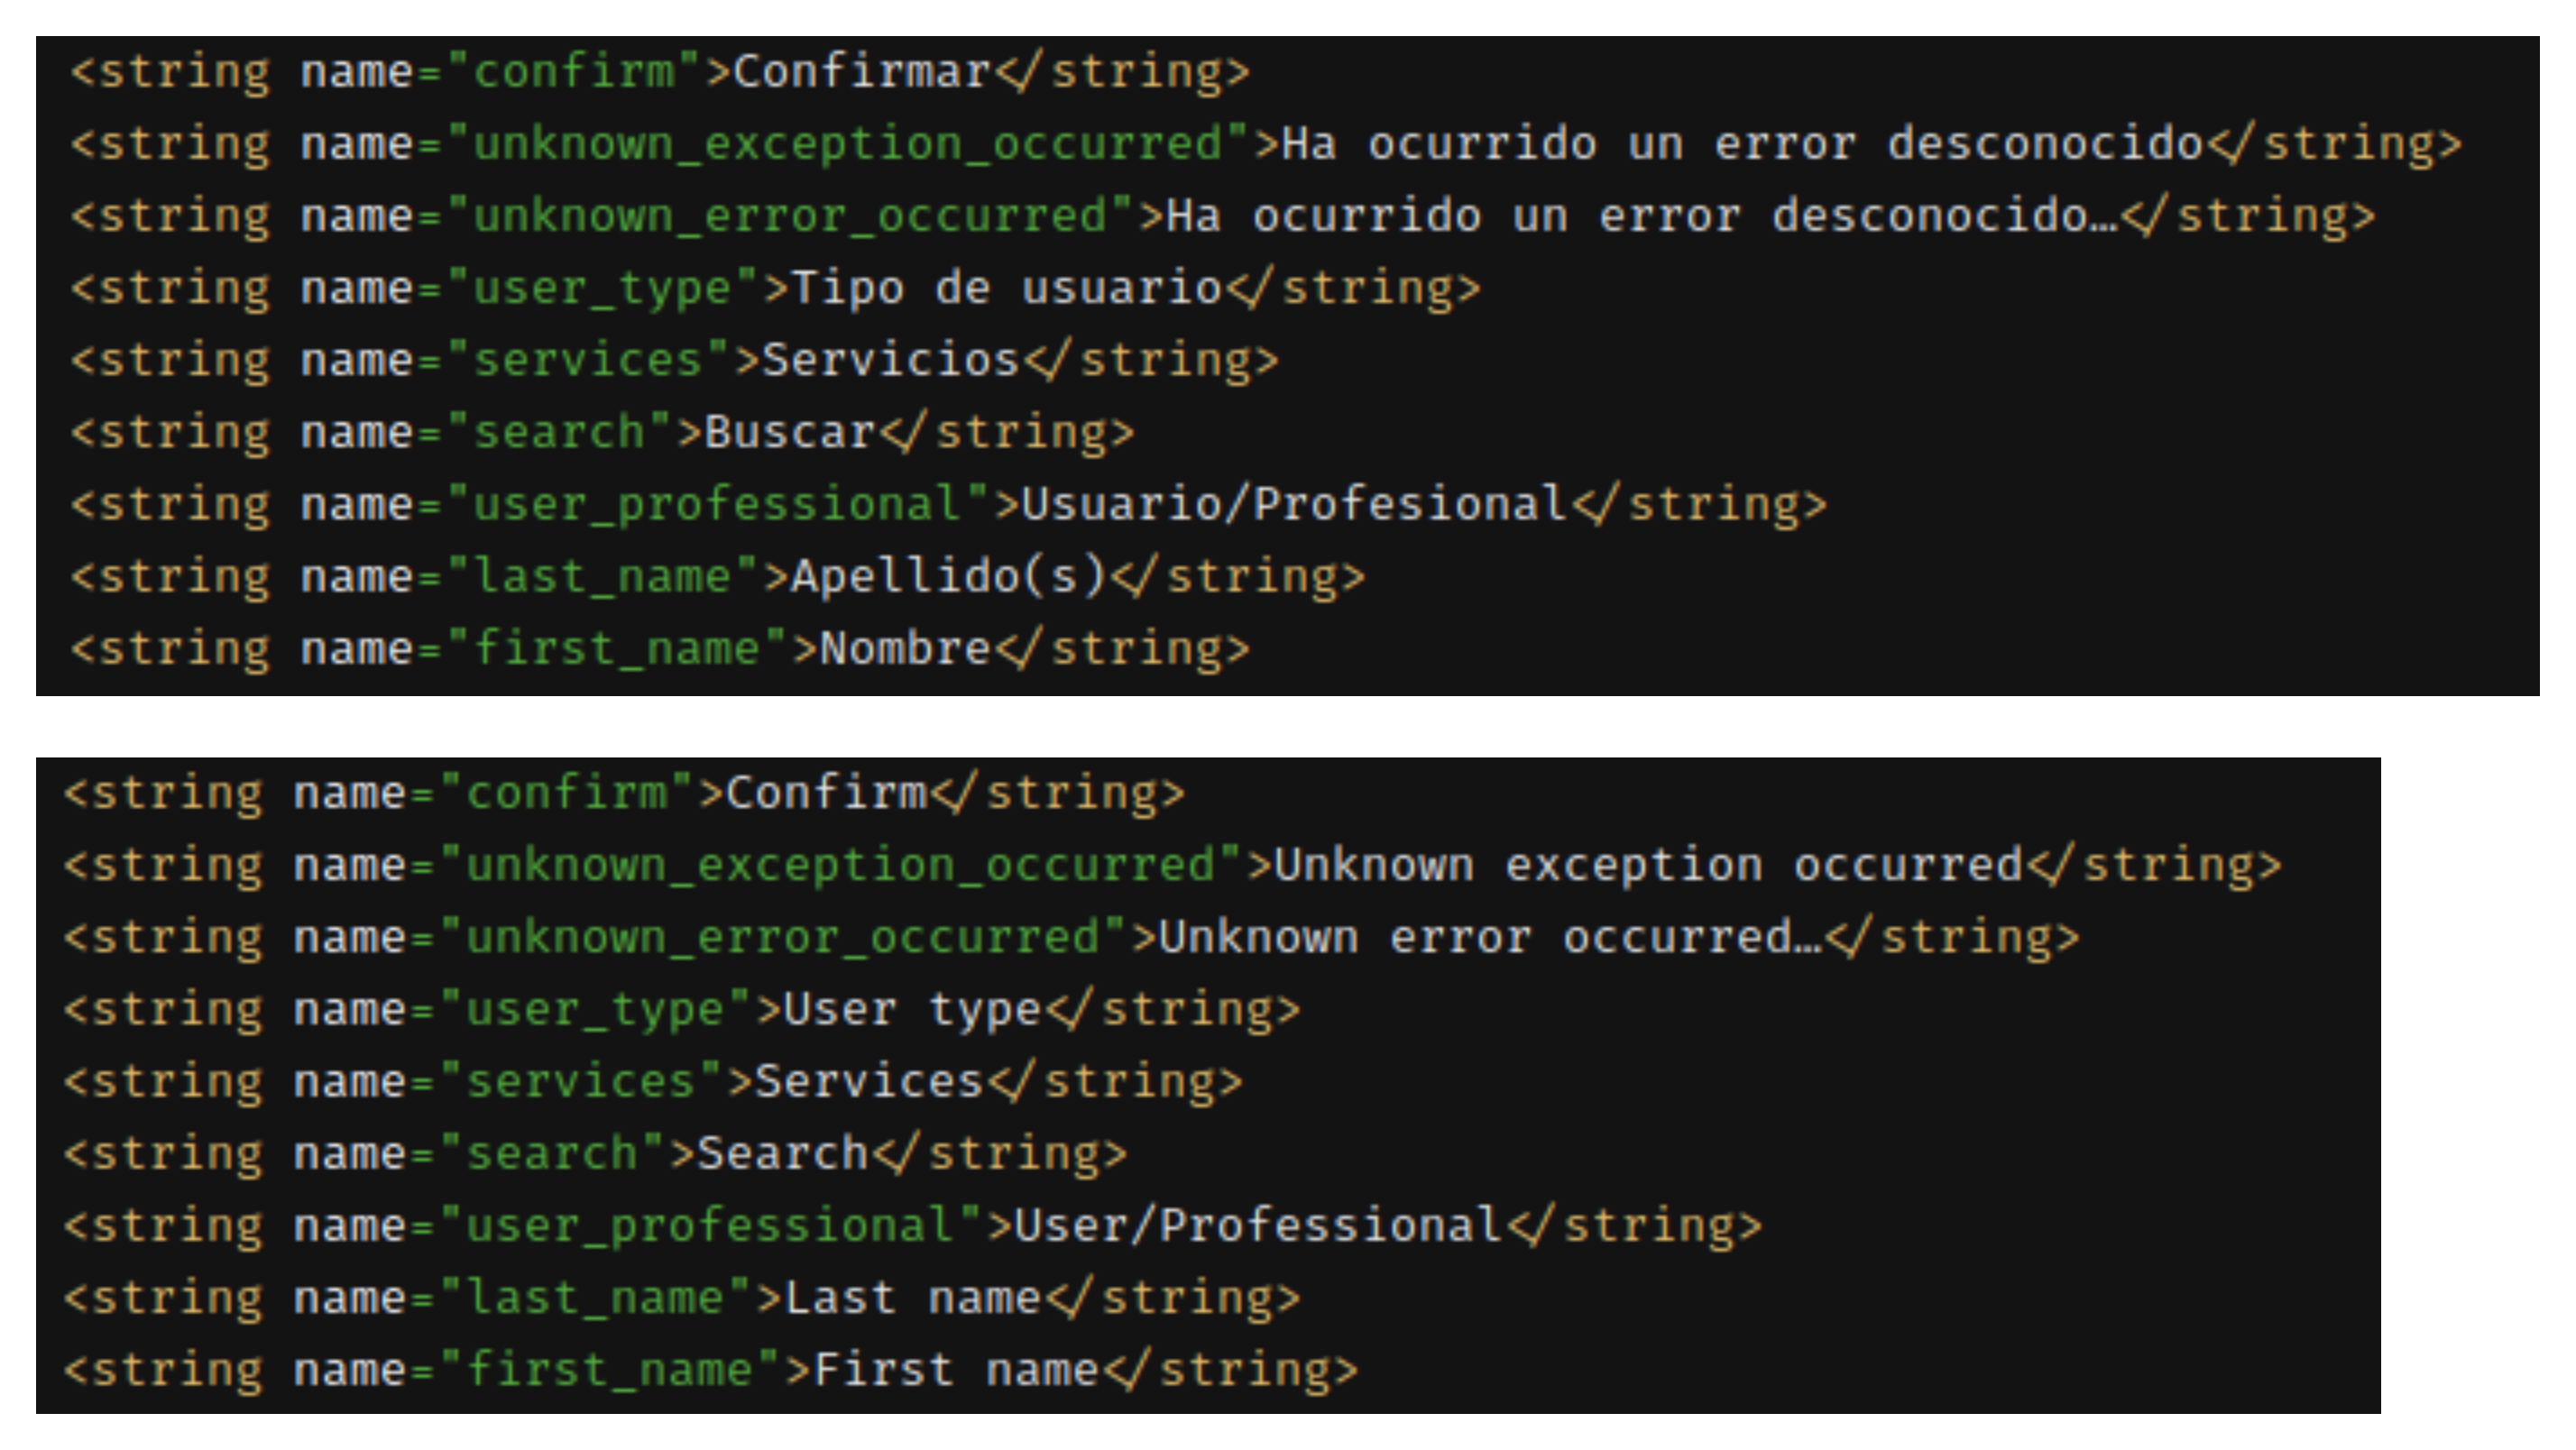
\includegraphics[width = 0.7\textwidth]{Imagenes/Fuentes/stringsXml.png}
    \caption{Parte del fichero strings.xml en su versión en inglés y español.}
    \label{fig:stringXml}
\end{figure}

\section{Implementación}
La implementación se ha dividido en cinco grupos con funcionalidades relacionadas: autenticación, usuarios y profesionales, trabajos y servicio; y chat. De cada grupo se explicarán las consideraciones fundamentales que se han tenido en cuenta a nivel de código. También se explicará con detalle el sistema de gestión de errores que ha sido utilizado por todos los bloques.
\subsection{Autenticación} 
Este bloque incluye las funcionalidades de inicio de sesión, registros, cierre de sesión y mantenimiento de sesión iniciada. Todas estas implementaciones han utilizado Firebase authentication (\ref{subsec:firebaseAuth}) como servicio de \textit{backend}.

El incio de sesión y el registro han sido implementados usando formularios para los campos requeridos, para ello se han utilizado \textit{Textfields}, un componente que ofrece Compose para el \textit{input} de cadenas de texto. También se ha comprobado que la cadena introducida por el usuario era correcta de forma dinámica (véase la figura \ref{fig:textfield}). 
\begin{figure}[h]
    \centering
    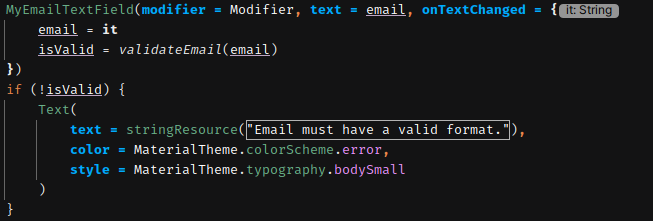
\includegraphics[width = 0.6\textwidth]{Imagenes/Fuentes/textfield.png}
    \caption{Ejemplo de validación del campo email.}
    \label{fig:textfield}
\end{figure}

El mantenimiento de la sesión sirve para que el usuario no tenga que iniciar sesión cada vez que abra la aplicación, sino que esta se guarda durante un tiempo determinado (en caso de cierre de sesión se elimina). Para ello se ha utilizado la \textit{Splash Screen}, de tal forma que al entrar en la aplicación, se comprueba si existe sesión, si existe, se redirige al usuario a la \textit{home}, sino, se le redirige a la pantalla de inicio de sesión (como se muestra en la figura \ref{fig:splashDest}). 
\begin{figure}[h]
    \centering
    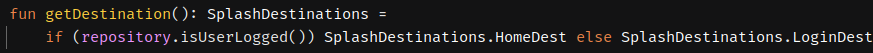
\includegraphics[width = 1\textwidth]{Imagenes/Fuentes/splashDest.png}
    \caption{Función que comprueba si hay una sesión guardada.}
    \label{fig:splashDest}
\end{figure}

\subsection{Usuarios y profesionales} 
Este bloque incluye las funcionalidades de perfil, editar datos, vista de perfil, lista de favoritos y búsqueda.

En la pantalla de perfil se ha implementado también la funcionalidad de cambio de tema de la aplicación. Los datos se han persistido utilizando un \textit{Singleton} (ver el apartado \ref{subsec:singletonComoModelo}), gracias a esto, los datos se sacan de Firestore al iniciar sesión, y se mantienen un tiempo limitado tras el cual se vuelven a sacar de remoto, esto consigue una actualización frecuente (si por ejemplo cambias los datos de la misma cuenta con otro dispositivo). Esta implementación también ha sido utilizada para la lista de favoritos. 

Para la función de ver el perfil de otro usuario también se ha seguido este método pero con motivación distinta, el objetivo era evitar que si un usuario pulsaba el botón de ver un perfil, luego se salía y volvía a pulsar en el mismo se llamara dos veces al servicio remoto. Lo que se ha conseguido es que al pulsar un perfil para ver, este se cachee en el \textit{Singleton} por si se realiza la misma acción. En cambio si el siguiente perfil a ver es diferente, se vacía la cache y se llena con el nuevo perfil.

A la hora editar los datos del perfil, se ha tenido en cuenta la implementación de estos \textit{Singletons}, ya que hay que asegurarse de que la copia en cache y en remoto se mantinenen sincronizadas. Esto supone un pequeño esfuerzo extra pero permite reducir el coste de llamadas remotas.

La búsqueda se ha implementado sacando el id, nombre completo, nombre de usuario, foto de perfil y tipo de actor de cada profesional. Cuando un item de la lista mostrada es pulsado, se saca la estructura de actor completa de base de datos usando el id de usuario y se muestra su perfil. 

\subsection{Trabajos y Servicios} 
Los trabajos se han dividido en 2 partes: solicitudes y trabajos en sí. Se han guardado como dos listas distintas para cada actor con los ids de los implicados, nombre de servicio, precio y nombre de usuario del otro actor implicado. Su implementación a nivel de código ha sido igual, variando solo en el lugar donde mostrar cada lista. Esto ha ahorrado mucho código duplicado. Se ha utilizado un \textit{booleano} como parámetro para diferenciar si se trata de una solicitud o un trabajo (ver figura \ref{fig:getJobOrRequest}).
\begin{figure}[h]
    \centering
    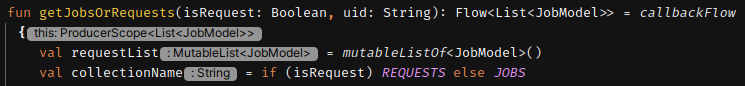
\includegraphics[width = 1\textwidth]{Imagenes/Fuentes/getJobOrRequest.png}
    \caption{Ejemplo de función condicionada por solicitud o trabajo.}
    \label{fig:getJobOrRequest}
\end{figure}

Por otro lado los servicios, que también se han implementado usando un \textit{Singleton} por las razones comentadas previamente, en la aplicación se utilizan como una lista de \textit{ServiceModel}, guardando el id del profesional al que pertenecen para poder ser clasificados. La lista de servicios mostrada recoge todos los servicios activos de la aplicación ya que por ahora el número no es demasiado grande, a pesar de esto, en el futuro se podrían filtrar y ordenar por otros atributos a parte del nombre o mostrar una lista con un máximo número de elementos a la que se le podrían ir añadiendo más (cargándolos de base de datos) a medida que el usuario atraviesa la lista.

\subsection{Chat} 
La implementación del modulo de Chat ha sido uno de los mayores desafíos de la aplicación a nivel lógico y de estructura de datos ya que en un comienzo, todos los modelos que se intentaron usar duplicaban muchos datos, haciendo la funcionalidad muy difícil de mantener. Al final se consiguió maximizar la eficiencia de las estructuras dividiendo la funcionalidad en dos colecciones (en el aprtado \ref{sec:modeloDatos} se explica el modelo de datos en detalle). 

Otro gran problema al inicio fue la necesidad de que todo se actualizara en tiempo real, para ello fue muy útil aunque difícil a nivel programático el uso de \textit{flows} (ver figura \ref{fig:flows_impl} como ejemplo de la implementación de flows) que en combinación con la capacidad reactiva de Jetpack Compose hicieron posible una latencia mínima.
\begin{figure}[h]
    \centering
    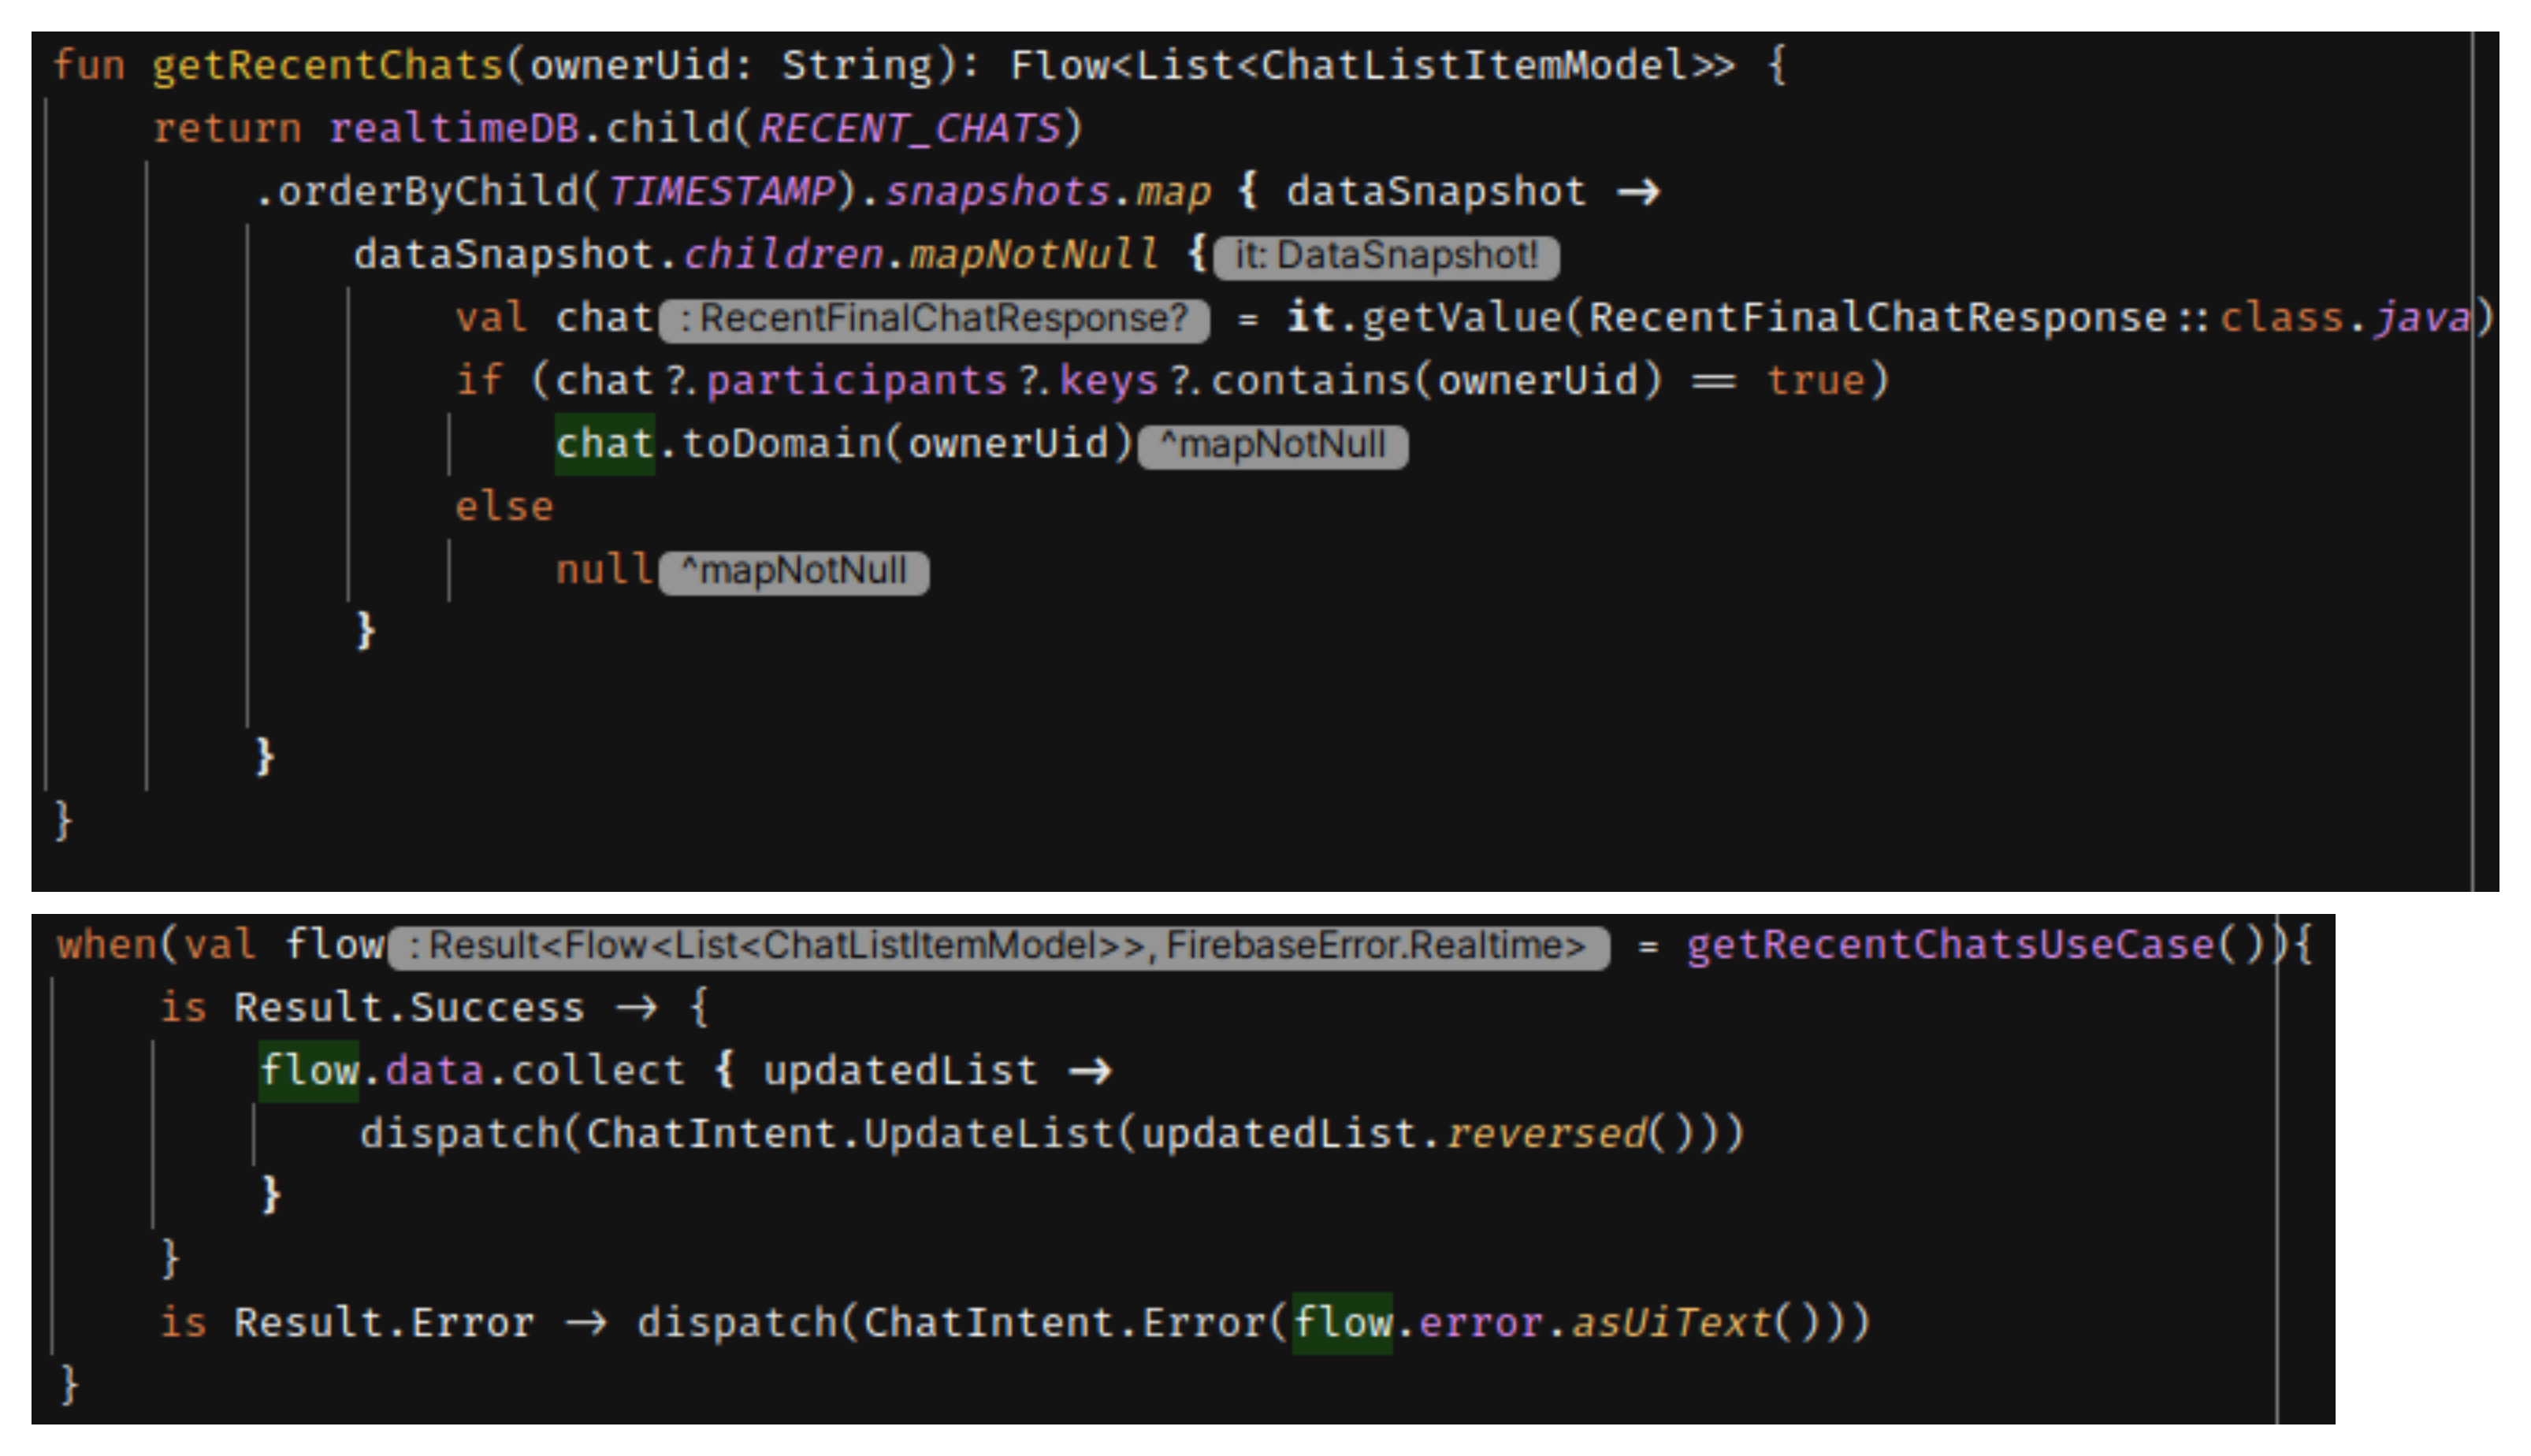
\includegraphics[width = 0.7\textwidth]{Imagenes/Fuentes/flows_impl.png}
    \caption{Ejemplo de uso de flows para sacar los chats recientes y recogerlos en el viewmodel.}
    \label{fig:flows_impl}
\end{figure}

\subsection{Gestión de errores} 
Para conseguir una gestión de errores eficiente y generalizada se han desarrollado una serie de clases, basadas en la estructura propuesta por el creador de contenido Philipp Lackner\hyperlink{cap:biblio}{\endnote{\textbf{Philipp Lackner on Error handling}: \url{https://www.youtube.com/watch?v=MiLN2vs2Oe0}}} y personalizadas según las necesidades específicas de la aplicación. Que en conjunto sirven como sistema bien estructurado que proporciona una forma cómoda de gestionar errores, respetando todos los principios de arquitectura limpia mencionados en el apartado \ref{subsec:cleanArch}. A continuación se explican todas las clases que se han creado, es posible que solo con la explicación que viene a continuación no se entienda el sistema en su totalidad, pero el lector tendrá disponible el código fuente para verlo aplicado y si es necesario clonar el repositorio para probarlo haciendo cambios.

En primer lugar se ha creado la interfaz \textit{Error}, mostrada en la figura \ref{fig:error_interface}, que no hará nada pero servirá para identificar todos los tipos de errores declarados.
\begin{figure}[h]
    \centering
    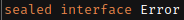
\includegraphics[width = 0.3\textwidth]{Imagenes/Fuentes/error_interface.png}
    \caption{Interfaz Error.}
    \label{fig:error_interface}
\end{figure}

En segundo lugar se ha creado la interfaz Result (se ha llamado así a pesar de que ya haya una clase con este nombre en la biblioteca estandar por considerarse el más apropiado). Esta es la interfaz principal que utilizan todas las funciones de la aplicación que devuelvan datos. Tiene dos parametros genéricos que cambiarán en cada caso específico -véase la figura \ref{fig:ejemplo_result}-, uno para los datos devueltos y otro para el tipo de error, también cuenta con los dos posibles resultados que pueda devolver una función que implemente esta interfaz: 
\begin{itemize}
    \item \textbf{Success}: para el caso de éxito. Llevará como parámetro los datos devueltos.
    \item \textbf{Error}: distinto de la interfaz explicada anteriormente, será lo que se devuelva en caso de error en la llamada a función y llevará como parámetro una clase que implemente la interfaz \textit{Error}.
\end{itemize}
\begin{figure}[h]
    \centering
    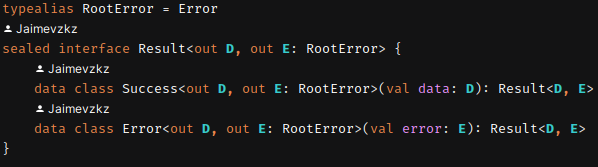
\includegraphics[width = 0.8\textwidth]{Imagenes/Fuentes/ejemplo_result.png}
    \caption{Interfaz Result.}
    \label{fig:ejemplo_result}
\end{figure}

Lo siguiente será crear tantas interfaces como sean necesarias -e implementen \textit{Error}- para cada tipo de error. En Profinder solo ha sido necesario crear una que englobara todos los errores relativos a \hyperlink{subsec:firebase}{Firebase}, sin embargo, es un sistema escalable a futuro.

Dentro de cada una de estas interfaz se declaran todos los tipos de errores (relativos a \hyperlink{subsec:firebase}{Firebase} por ejemplo, véase la figura \ref{fig:ejemplo_tipo_error}) como clases enumeradas, consiguiendo así que cada uno sea un enumerado que se gestiona de forma independiente en las distintas capas de la aplicación.
\begin{figure}[h]
    \centering
    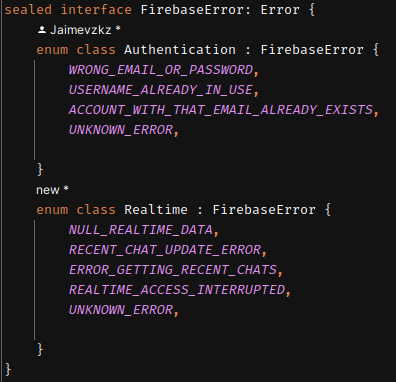
\includegraphics[width = 0.7\textwidth]{Imagenes/Fuentes/ejemplo_tipo_error.png}
    \caption{Ejemplo de tipo de error.}
    \label{fig:ejemplo_tipo_error}
\end{figure}

Con todo lo anterior, la gestión de errores se convierte en algo sencillo, las funciones deberán devolver un tipo \textit{Result} (figura \ref{fig:ejemplo_impl_result}).
\begin{figure}[h]
    \centering
    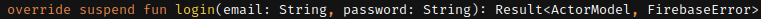
\includegraphics[width = 0.9\textwidth]{Imagenes/Fuentes/ejemplo_impl_result.png}
    \caption{Ejemplo de implementación de Result.}
    \label{fig:ejemplo_impl_result}
\end{figure}

Y en las llamadas a función se podrá gestionar si hay un error dividiendo los casos con una expresión
\textit{when}\hyperlink{cap:biblio}{\endnote{\textbf{when}: \url{https://www.programiz.com/kotlin-programming/when-expression}}}, como se ve en lafigura \ref{fig:llamada_funcion_result}.
\begin{figure}[h]
    \centering
    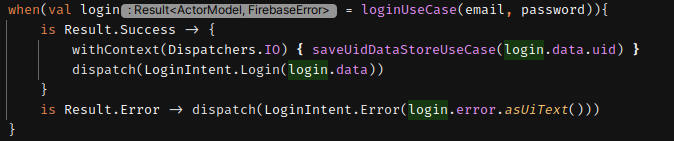
\includegraphics[width = 0.8\textwidth]{Imagenes/Fuentes/llamada_funcion_result.png}
    \caption{Ejemplo de llamada a función implementando Result.}
    \label{fig:llamada_funcion_result}
\end{figure}